\subsection{Phase 1 Achievements and Phase 2 Objectives}

\begin{figure}[H]
    \centering
    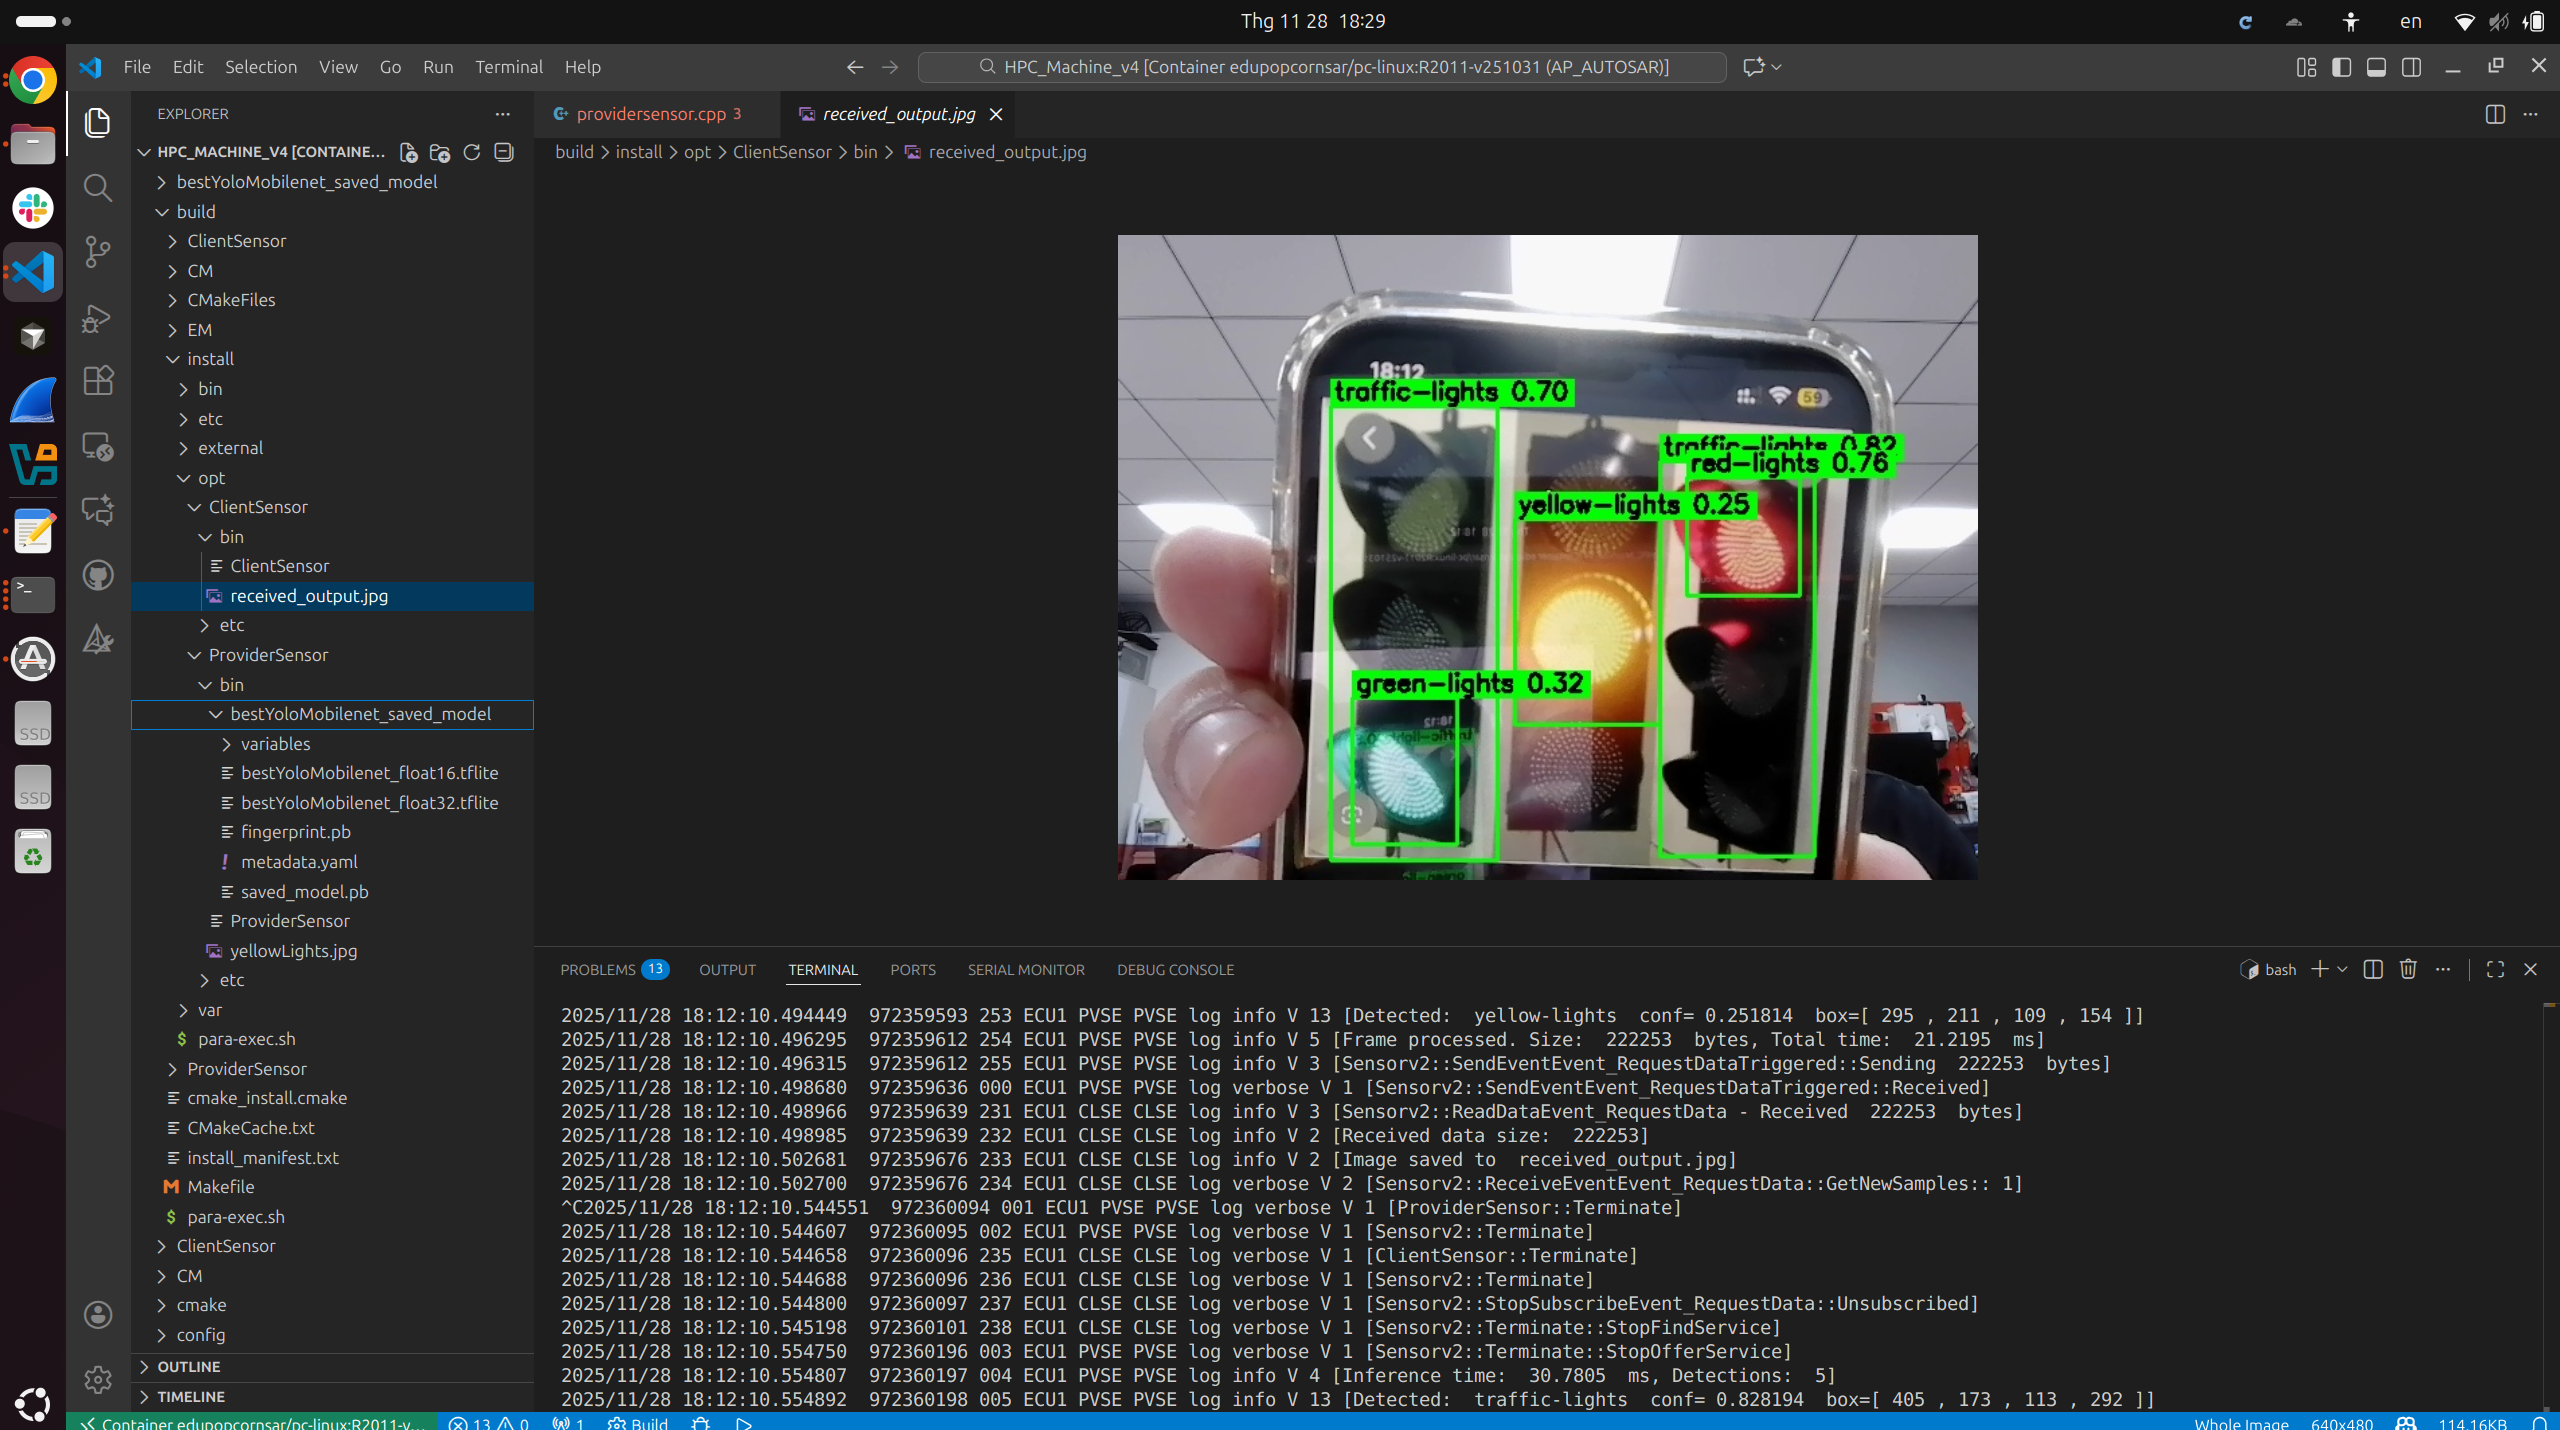
\includegraphics[width=0.75\textwidth]{Images/resultPhrase1.png}
    \vspace{0.5cm}
    \caption{The result of the prototype project in Phase 1}
    \label{fig:res_project_phase1}
\end{figure}

As illustrated in Figure~\ref{fig:res_project_phase1}, the first phase of this project successfully established the foundational architecture for an edge-based perception system. The Adaptive AUTOSAR platform was deployed and executed within a Docker container environment, proving the viability of containerized automotive software. For the visual perception task, a YOLO11n-MobileNetV4 model was utilized to perform basic traffic light detection, limited primarily to identifying red, yellow, and green signal states. The processed sensor data was transmitted seamlessly between applications via the SOME/IP communication middleware, successfully validating the basic service-oriented data flow. Following the successful completion of Phase 1, the core findings and architectural methodologies were compiled into a research paper submitted to the IEEE Sensors Applications Symposium 2026 (IEEE SAS 2026). This manuscript, scheduled for presentation in July 2026, is provided in full in \hyperref[chap:append]{Appendix}.

Building upon that success, the current and final phase of the project significantly upgrades both the software architecture and the perception capabilities. The Adaptive AUTOSAR configuration is transitioned to utilize the Data Distribution Service (DDS) middleware, providing a more robust communication backbone and also following the ADAS standards. The perception pipeline is completely overhauled by replacing the YOLO11 baseline with the newest Ultralytics architecture, chosen specifically for its anchor-free and Non-Maximum Suppression (NMS)-free design. To handle complex intersection data, a custom lightweight multi-head CNN is introduced to explicitly detect countdown timers, while the GPS module is integrated to cross-reference Intelligent Transportation Systems (ITS) nodes for early, predictive warnings. Ultimately, these enhancements expand the detection scope from simple color recognition to identifying specific lane directions, signal colors, and timer values simultaneously, all while maintaining high accuracy and an inference speed of $\geq 15$ frames per second (FPS) in edge device, which completely run on CPU without GPU and NPU. And the next section, we will introduce the contribution and structure of our report.

\section{Contributions and Report Structure}

The preceding sections have established the foundational context for the proposed red-light warning system. By exploring the background of traffic safety and the limitations of current solutions, the core motivation for this project has been clearly defined. Furthermore, the specific system requirements, project scope boundaries, and related research gaps have also been outlined.

To address these identified challenges, this project makes two major technical contributions:
\begin{enumerate}
    \item \textbf{Implementing Adaptive AUTOSAR to Industry Standards:} The project successfully develops and deploys a service-oriented software architecture using the PopcornSAR toolchain. This implementation closely follows modern automotive industry standards, ensuring robust and reliable inter-process communication.
    \item \textbf{Deploying Edge AI on Constrained Hardware:} The project designs a highly optimized, lightweight AI perception pipeline (utilizing a YOLO-MobileNetV4 and multi-head CNN architecture). This pipeline is capable of running efficiently on an edge device to achieve real-time traffic light detection without relying on high-end cloud computing.
\end{enumerate}

With the problem clearly defined and the main contributions established, the remainder of this report is logically structured to guide the reader through the technical development of the project. The subsequent chapters are organized as follows:

\begin{itemize}
    \item \textbf{Chapter 2 (Related Works):} Reviews existing literature to provide a critical context for the research. It explores current traffic light detection methods, the practical challenges of deploying complex AI models on edge devices, and the role of GNSS positioning in modern automotive systems.
    
    \item \textbf{Chapter 3 (Background):} Introduces the fundamental technologies that form the foundation of the project. It clarifies the core concepts of the Adaptive AUTOSAR framework, alongside the selected perception tools such as the YOLO algorithm and the LiteRT inference engine.
    
    \item \textbf{Chapter 4 (System Configuration and Methodology):} Details the software setup and the proposed development workflow. It thoroughly explains the design of service-oriented interfaces, the training processes for the customized YOLO-MobileNetV4 and Multi-head CNN models, and the creation of a reproducible execution environment.
    
    \item \textbf{Chapter 5 (Project Prototype):} Demonstrates the actual hands-on implementation of the ADAS system. It traces the complete data flow from sensor acquisition to the driver display using DDS middleware, while also presenting the final experimental setup and evaluation results.
    
    \item \textbf{Chapter 6 (Conclusion and Future Enhancement of Project):} Concludes the thesis by summarizing the primary achievements and evaluating the system's overall effectiveness. It reflects on the prototype's real-world performance and outlines potential avenues for future research.
\end{itemize}

Together, this structure ensures a clear and comprehensive progression from the initial problem statement to a fully functioning driver assistance system.
